\chapter{Analýza a návrh herního systému}
\label{chap:design_analysis}

Pro rozumný vývoj herního systému modelové hry je nutné nejprve provést analýzu a návrh, proto se tato kapitola tímto tématem zabývá. První část se zaměřuje na požadavky, které by měl herní systém splňovat, druhá část se pak věnuje samotnému návrhu herního systému.

Hybridní deskové hře, která je finálním produktem této práce, bylo určeno pracovní jméno \textit{Trails Through Shadows} (zkratkou \textit{TTS}). Dále je však zmiňována především pod názvem \textit{modelová hra}.



\section{Požadavky na modelovou hru}
\label{sec:requirements}

Před samotným návrhem herního systému je nutné stanovit požadavky, které by měl herní systém a hra jako taková splňovat. Tyto požadavky byly stanoveny na základě analýzy existujících řešení \chapterref{chap:game_analysis} a vlastních představ týmu a byly rozděleny do následujících kategorií.

\subsection{Struktura hry}
\label{subsec:req_structure}

\begin{itemize}
    \item \textbf{Kooperace} -- 
        Hra by měla být kooperativní, tedy hráči by měli spolupracovat na dosažení cíle hry společně.
    \item \textbf{Příběh} -- 
        Hra by se měla držet centrálního příběhu, který hráče zaujme a bude je v průběhu hry motivovat.
    \item \textbf{Jedinečnost postav} -- 
        Hráči by měli být schopni vytvořit jedinečnou postavu, která se od ostatních liší nejen vzhledem, ale i herním stylem.

    \begin{itemize}
        \item \textbf{Unikátní akce} -- 
            Postavy by měly mít akce, které jsou pro ně specifické a mají velký vliv na pocit, který hráči z postavy mají.
        \item \textbf{Jiné statistiky} -- 
            Statistiky jsou další oblastí, ve které by se postavy měly lišit.
        \item \textbf{Vývoj postav} -- 
            Postavy by měly mít možnost se vyvíjet, získávat nové schopnosti a zlepšovat své statistiky, ať už získáváním zkušeností nebo pomocí předmětů.
    \end{itemize}

    \item \textbf{Rozdělení na světovou a lokální mapu} -- 
        Herní svět bude zobrazen ve velké mapě v rámci webové aplikace, která bude obsahovat jednotlivé lokace. Ty budou mít svou vlastní mapu, která bude detailnější a bude sloužit pro souboje a interakci s prostředím.
    \item \textbf{Propojení s aplikací} -- 
        Hra bude propojena s webovou aplikací, která bude sloužit pro zjednodušení hraní hry a bude obsahovat informace, které by byly obtížné zobrazit ve fyzických komponentách. Je však nutné dbát na to, aby si hra zachovala svůj deskový charakter.
\end{itemize}

\subsection{Herní mechaniky}
\label{subsec:req_mechanics}

\begin{itemize}
    \item \textbf{Karty a kostky} -- 
        Souboj by měl být založen na kartách, které budou hráči umožňovat provádět různé akce, a kostkách, které budou přinášet do výsledku náhodnost.
    \item \textbf{Příběh} -- 
        Příběh bude vyprávěn především prostřednictvím webové aplikace.
    \item \textbf{Inventář a předměty} -- 
        Předměty budou důležitou součástí hry díky jejich vlivu na vylepšení postavy. Inventář bude sloužit k jejich ukládání a bude omezený na typy předmětů.
    \item \textbf{Efekty} -- 
        Hra by měla obsahovat efekty, které mohou ovlivňovat hráčské postavy nebo nepřítele.
\end{itemize}

\subsection{Komponenty}
\label{subsec:req_components}

\begin{itemize}
    \item \textbf{Kostky} -- 
        Kostky budou sloužit k určení výsledku útoků a jiných akcí, které hráči provádějí. Na stěnách kostky budou zaznamenány modifikátory ovlivňující výsledek a každý hráč bude mít svůj vlastní kostku.
    \item \textbf{Karty} --
        Karty budou reprezentovat akce v rámci hry a budou obsahovat strukturované informace o tom, jak se daná akce provádí a jaké má následky.
    \item \textbf{Figurky} --
        Postavy, nepřátelé, summoni a překážky budou reprezentovány figurkami, z důvodu omezeného rozpočtu se však bude jednat o \textit{standees}.
    \item \textbf{Mapy lokací} --
        Lokace se bude skládat z jednotlivých menších částí, které bude možné skládat dohromady a spojovat do většího celku. Mapa bude založena na hexagonech.
    \item \textbf{Pravidla} --
        Pravidla budou zapsána ve vytištěné příručce přiložené jako součást balení hry, ale budou také dostupná v elektronické podobě. Hráče provedou průběhem hry a jednotlivými mechanismy v přehledné a graficky přívětivé formě.
    \item \textbf{Přizpůsobení pro webovou aplikaci} --
        Webová aplikace bude neodlučitelnou součástí hry, bude vytvořena primárně pro desktopové zařízení s možností responzivního designu pro mobilní zařízení. Bude obsahovat informace o postavách, lokacích, předmětech a dalších herních prvcích, které by byly obtížné zobrazit ve fyzické podobě a bude dbáno na grafickou koherenci s fyzickými komponentami.
\end{itemize}

\subsection{Komerční aspekty}
\label{subsec:req_commercial}

\begin{itemize}
    \item \textbf{Cílová skupina} --
        Hra bude určena pro hráče, kteří již mají zkušenosti s deskovými hrami podobného stylu, ale zároveň bude přístupná i pro nováčky, kteří se chtějí do světa deskových her dostat.
    \item \textbf{Jednoduchost výroby} --
        Hra bude navržena tak, aby byla jednoduchá na výrobu.
    \item \textbf{Cena hry a aplikace} --
        Cena hry bude nastavena tak, aby byla dostupná pro většinu hráčů, ale zároveň aby bylo možné z ní pokrýt náklady na výrobu a distribuci. Webová aplikace bude dostupná zdarma po zadání licenčního klíče fyzické hry.
    \item \textbf{Rozšíření} --
        Hra bude navržena tak, aby bylo možné v budoucnu vytvořit rozšíření, které by přidalo nové postavy, lokace a příběh.
\end{itemize}



\section{Návrh herního systému}
\label{sec:design}

Na základě požadavků stanovených v předchozí sekci byl vytvořen návrh herního systému, je pro přehlednost rozdělen do několika částí. První část se zabývá herními mechanikami, druhá část se zaměřuje na komponenty hry a třetí část se věnuje propojení s webovou aplikací.

\subsection{Schéma hry}
\label{subsec:design_scheme}

\textbf{// TODO zjednodušený ER diagram databáze}

\subsection{Herní mechaniky}
\label{subsec:design_mechanics}

Mechaniky modelové hry jsou silně inspirované především výše zmíněnou deskovou hrou \glsref{gloomhaven}, ale jsou upravené tak, aby lépe vyhovovaly výše stanoveným požadavkům. 

\subsubsection*{Souboj}
\label{subsubsec:encounter}

\begin{figure}[H]
    \centering
    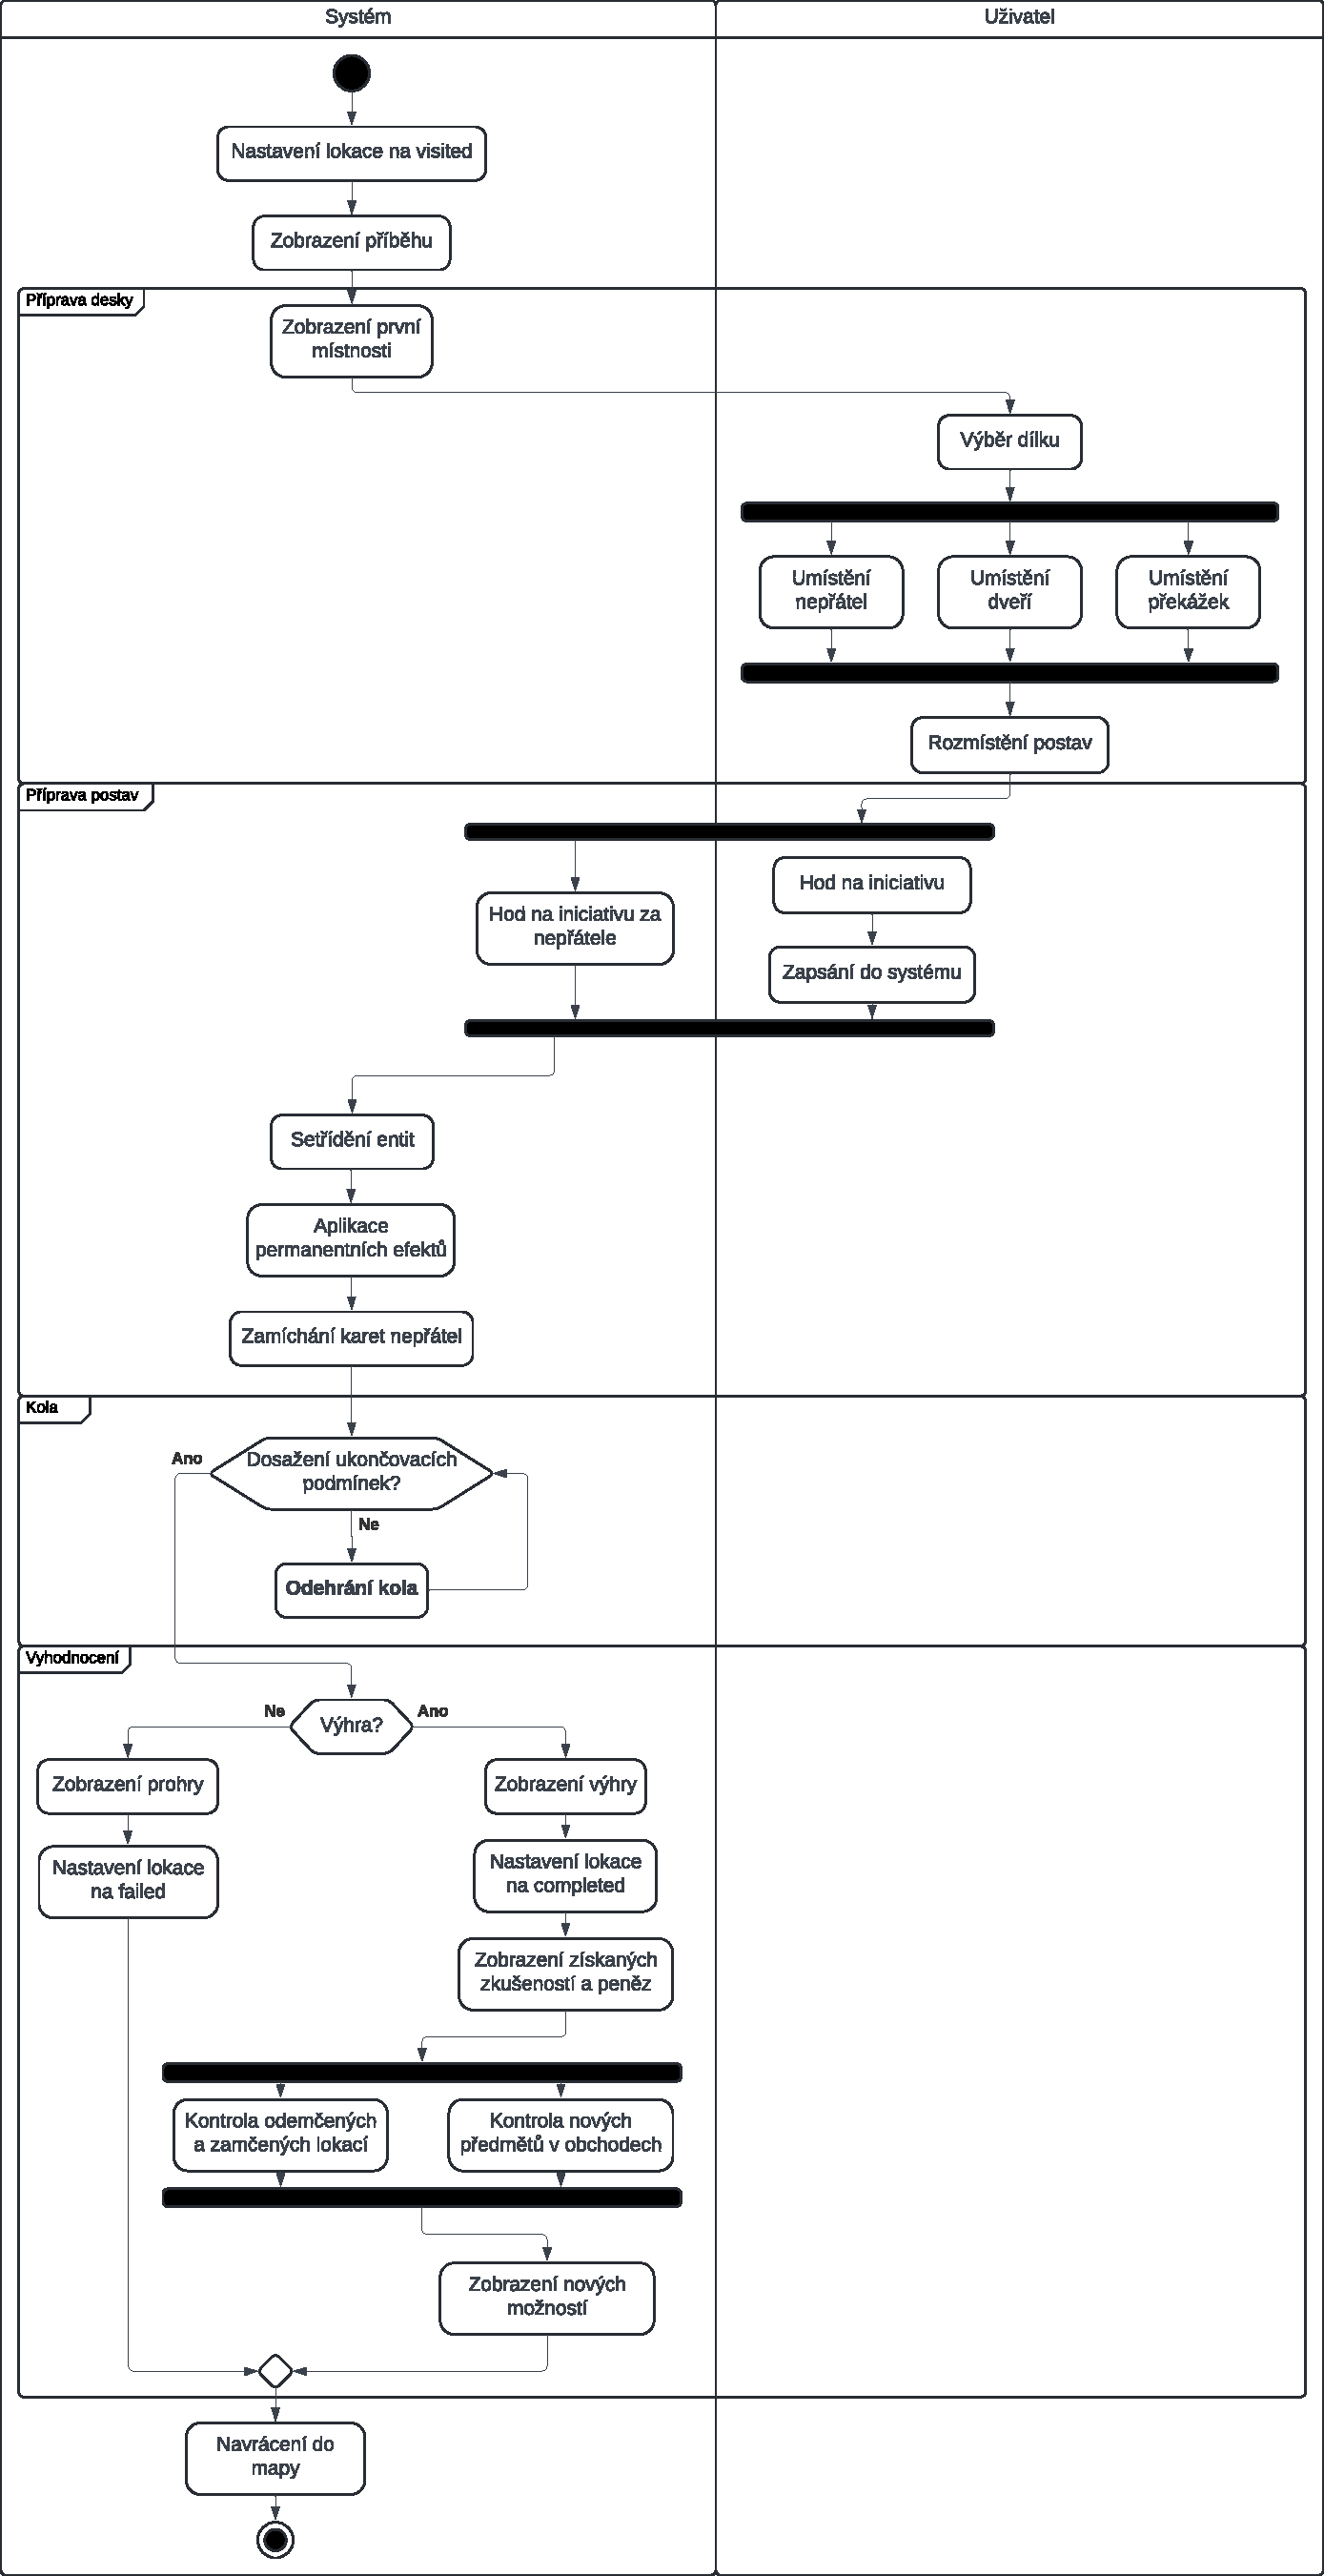
\includegraphics[height=0.9\textheight]{figures/diagrams/encounter.pdf}
    \caption{Diagram průchodu lokací}
    \label{diag:encounter}
\end{figure}

Souboj je hlavní funkcionalitou, kterou hra nabízí. Průběh souboje je rozdělen do několika fází, které jsou znázorněny na diagramu \ref{diag:encounter}. Ještě před samotným hraním si systém zaznačí, že lokace už byla navštívena (\texttt{visited}), pokud již nemá nastavený jiný stav, který je důležitější (jako například \texttt{completed} nebo \texttt{failed}). Následně hráčům zobrazí příběh, který je s touto lokací spojený.

Poté následuje fáze přípravy hrací desky. Systém zobrazí počáteční místnost lokace, všechny nepřátele, překážky a dveře, které se v ní vyskytují spolu s identifikátory, které umožní hráčům tyto části jednoduše najít a sestavit tak odpovídající konfiguraci místnosti na herním stole. Když je všechno připraveno, hráči umístí své postavy na políčka určená pro hráče a s tím je příprava herního pole hotová.

Druhá část přípravy je věnována samotným postavám a nepřátelům a tvorbě iniciativního žebříčku. Každý s hráčů si hodí svou kostkou na iniciativu a zaznamená výsledek do systému, který tento modifikátor automaticky přičte k základní výši iniciativy, který hráčova postava získala ze své rasy, třídy a vybavení. Za nepřátele toto provede systém automaticky. Výsledný žebříček je seřazen sestupně a hráči a nepřátelé se podle něj střídají v rámci kola. Dále se tu také provádí aplikace permanentních efektů, tedy efektů získaných ze zázemí a předmětů u postav nebo vrozené efekty u nepřátel, podle diagramu \textbf{//TODO}. Systém pak ještě zamíchá simulovaný balíček nepřátelských karet, který bude sloužit k určení jejich akcí.

Následuje fáze kol, která se provádí podle diagramu \textbf{//TODO} opakovaně ve smyčce, dokud hráči nesplní jistou předem určenou ukončovací podmínku.

Po dosažení této podmínky systém vyhodnotí, jak hra skončila. Pokud se jedná o prohru, zobrazí tuto informaci hráčům a nastaví stav lokace na \texttt{failed}. Pokud ovšem hráči lokaci zdolali úspěšně, systém provede kontrolu nových lokací a předmětů v obchodech, které hráči dokončením tohoto souboje odemkli nebo naopak zablokovali. Pomocí tohoto mechanismu se zajišťuje, že hra bude mít dynamický průběh a hráči budou mít motivaci prozkoumávat nové lokace a plnit úkoly. Po této kontrole systém hráčům zahlásí co vše jejich úspěch změnil, jaké mají nové možnosti a kolik peněz a zkušeností svou výhrou získali. Na závěr systém přehraje příběh konce této lokace a navrátí hráče zpět do mapy, kde mohou pokračovat v průzkumu světa.

\subsubsection*{Kola}
\label{subsubsec:rounds}

\begin{figure}[h]
    \centering
    \includeplantuml[scale=0.7]{round}
    \caption{Diagram kola}
    \label{diag:round}
\end{figure}

V rámci herního kola se nejprve provádí tahy hráčů a nepřátel v pořadí iniciativy podle diagramů \ref{diag:player_turn} a \ref{diag:enemy_turn}. Když tahy dojdou na konec iniciativy, systém zkontroluje, zda některý z hráčů během svého kola neotevřel dveře. Pokud ano, pak je hráčům zobrazena nově odhalená místnost, jejíž desku, nepřátele, překážky a dveře si opět podle identifikátorů rozloží na herní stůl, čímž se herní plocha rozšíří. Systém následně přidá nové nepřátele do iniciativního žebříčku a zamíchá jejich karty. Pokud hráči dveře neotevřeli, systém přeskočí tuto fázi, po které již kolo končí.


\subsubsection*{Tahy}
\label{subsubsec:turns}

\begin{figure}[h]
    \centering
    \includeplantuml[scale=0.7]{playerTurn}
    \caption{Diagram herního tahu hráče}
    \label{diag:player_turn}
\end{figure}

Tah hráče je vyobrazen na diagramu \ref{diag:player_turn}. Během začátku a konce se systém věnuje efektům, jejichž vyhodnocení a uvolnění je popsáno v diagramach \textbf{//TODO} a \textbf{//TODO}, což uvolňuje čas, který by jinak musel být stráven jejich monitorováním. Samotný hráč má nejprve za úkol vybrat si dvě karty, které v tomto kole bude chtít zahrát. Následně akce na kartách vyhodnotí podle diagramu \textbf{//TODO} a pokud má vyvolané nějaké summony, zahraje také jejich akce. Veškeré akce může vykonat v libovolném pořadí, což mu dává možnost plánovat své tahy tak, aby byly co nejefektivnější. Pokud během vykonávání akcí dojde k změně stavu jakékoliv entity na herní desce, hráč tyto změny zaznamená a pokračuje v dalších akcích. Po vykonání všech akcí hráč zahodí zahrnuté karty podle jejich zahazovacího pravidla, čímž své kolo ukončí.

\begin{figure}[h]
    \centering
    \includeplantuml[scale=0.7]{enemyTurn}
    \caption{Diagram herního tahu nepřítele}
    \label{diag:enemy_turn}
\end{figure}

Tah nepřítele znázorněn na diagramu \ref{diag:enemy_turn} je oproti tomu hráčskému mnohem jednodušší. Nepřátelé mají svůj vlastní balík karet, ze kterého jim systém vybere jednu, kterou v daném kole zahrají. Jedná se o simulaci reálného karetního balíčku, takže pokud v něm karty dojdou, opět se všechny zamíchají a tahají se znova. Na hráčích pak závisí, aby vyhodnotili, jakým způsobem se nepřátelé pohnou a na koho zaútočí, ale musí se řídit instrukcemi, které od systému dostali. Jakékoli změny musí být opět propsány do systému, který se zde také stará o vyhodnocení efektů.


\subsubsection*{Akce}
\label{subsubsec:actions}


\subsubsection*{Efekty}
\label{subsubsec:effects}

// aplikace efektu
// vyhodnocení efektu
// uvolnění efektu